\par $S = [6,6]$

\vskip 0.1in
\par $S_{alternativa^+} = [3,3]$   \qquad $S_{alternativa^-} = [3,3]$
\par $Ganho(S, S_{alternativa}) = 0$

\vskip 0.1in
\par $S_{bar^+} = [3,3]$  \qquad $S_{bar^-} = [3,3]$
\par $Ganho(S, S_{bar}) = 0$

\vskip 0.1in
\par $S_{fimSemana^+} = [2,3]$  \qquad $S_{fimSemana^-} = [4,3]$
\par $Ganho(S, S_{fimSemana}) = 0.02$

\vskip 0.1in
\par $S_{fome^+} = [5,2]$ \qquad   $S_{fome^-} = [1,4]$
\par $Ganho(S, S_{fome}) = 0.158$

\vskip 0.1in
\par $S_{clientes^{alg}} = [4,0]$  \qquad $S_{clientes^{cheio}} = [2,4]$ \qquad $S_{clientes^{nin}} = [0,2]$
\par $Ganho(S, S_{clientes}) = 0.540$

\vskip 0.2in
\par $S_{preco^{S}} = [3,4]$  \qquad $S_{preco^{SS}} = [2,0]$ \qquad $S_{preco^{SSS}} = [1,2]$
\par $Ganho(S, S_{preco}) = 0.195$

\vskip 0.1in
\par $S_{chuva^{+}} = [3,2]$  \qquad $S_{chuva^{-}} = [3,4]$
\par $Ganho(S, S_{chuva}) = 0.02$

\vskip 0.1in
\par $S_{reserva^{+}} = [3,2]$  \qquad $S_{reserva^{-}} = [3,4]$
\par $Ganho(S, S_{reserva}) = 0.02$

\vskip 0.1in
\par $S_{tipo^{Fra}} = [1,1]$  \qquad $S_{tipo^{Tai}} = [2,2]$ 
    \qquad $S_{tipo^{Ita}} = [1,1]$ \qquad $S_{tipo^{Ham}} = [2,2]$ 
\par $Ganho(S, S_{tipo}) = 0$

\vskip 0.1in
\par $S_{tespera^{0-10}} = [4,2]$  \qquad $S_{tespera^{10-30}} = [1,1]$ 
    \qquad $S_{tespera^{30-60}} = [1,1]$ \qquad $S_{tespera^{>60}} = [0,2]$ 
\par $Ganho(S, S_{tespera}) = 0.207$

\vskip 0.25in
\hfil
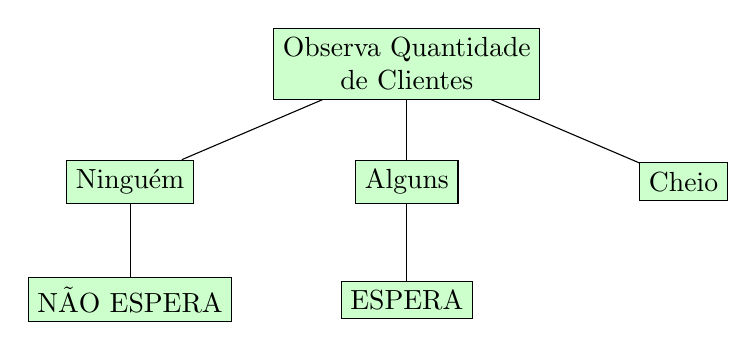
\begin{tikzpicture}[sibling distance=10em,
    every node/.style = {shape=rectangle, 
      draw, align=center,
      top color=green!20, bottom color=green!20}]]
    \node {Observa Quantidade \\ de Clientes}
        child { node {Ninguém} child { node {NÃO ESPERA}  } }
        child { node {Alguns} child { node {ESPERA} } }
        child { node {Cheio} };
  \end{tikzpicture}